\section{Hierarchical Hybrid Dataflow}
\label{sec:method}
The motivation leaves a central question unanswered. A useful local unit
must contain enough dependent work to reuse values, yet remain small enough
to admit a feasible mapping. Choosing a tile from its size alone does not
establish that its inputs are available or that its outputs can feed the next
tile. We therefore start with the dependencies and derive the execution units
before assigning resources to them.

The construction takes an \textbf{operator contract}
covering arithmetic, coefficients, direction, normalization, and logical
ordering, a \textbf{workload domain} covering shape, batch, placement, and
strides, and \textbf{hardware capabilities} covering resources and cores.
They specialize one construction rather than independent implementations.
We first derive closed subgraphs, then compose them across storage scopes,
and finally derive their communication and the conditions for reusing the
construction across variants. The 16-point Hadamard example introduced in
the motivation serves as a concrete instance throughout.

\subsection{Dependency-closed subgraphs}
Local reuse is possible only when a chosen group contains the values needed
by all of its internal operations. The stage-bit representation makes this
condition constructive rather than a property checked after arbitrary tiling.
\textbf{A stage band determines its local data domain.}
For a radix-two transform, choose a consecutive stage band and let $Q$
contain its pairing bits. Holding every other index bit fixed gives
\begin{equation}
\mathcal I(a,Q)=\{i\mid i\text{ agrees with }a\text{ outside }Q\}.
\label{eq:component}
\end{equation}
Every pair update in the band changes only a bit in $Q$ and thus stays inside
this component. Assignments to the fixed bits partition the array into
independent components of $2^{|Q|}$ values. The band's computation on one
component is a \textbf{dependency-closed subgraph}. Closure is local to the
band, whose inputs and outputs still connect to other bands.

Any ordered stage partition defines such components. Band width controls local
reuse, while the number of components assigned to a worker controls worker
reuse. Arithmetic labels remain attached to the operations. In particular,
an FFT band may require global-index-dependent twiddles, so a standalone
smaller FFT is not automatically a compatible core.

\noindent\textbf{A running example.}
For a 16-point unnormalized Hadamard transform with stage bits $(0,1,2,3)$,
write $i=4r+c$. Two equal bands give four row subgraphs varying $c$, then
four column subgraphs varying $r$. Each uses a four-point Hadamard core.
This instantiates the two-band case in
Figure~\ref{fig:organization-tradeoffs}. The component boundary follows
which bits vary, not whether the values happen to be contiguous in the
original array. The implementation can therefore choose a representation
that matches its store and read constraints without changing the logical
computation.

\begin{figure}[t]
\centering
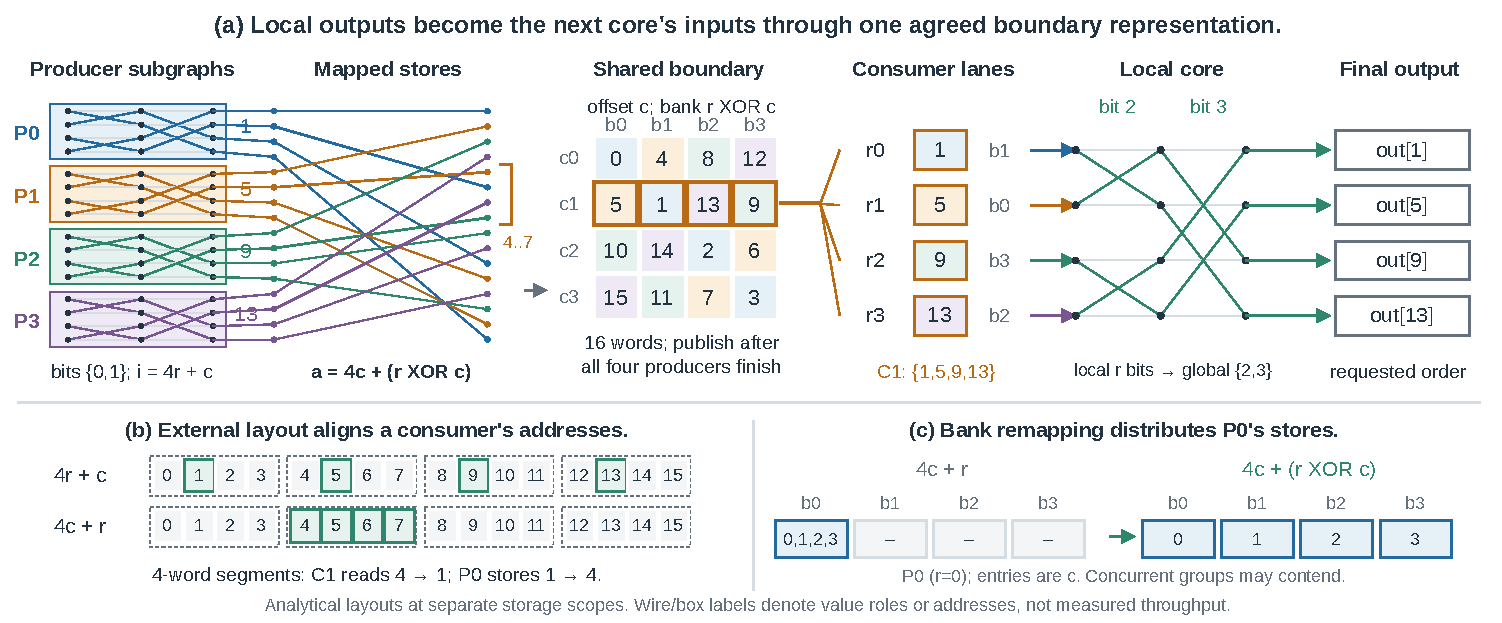
\includegraphics[width=\columnwidth]{figures/drawio/exports/hierarchy.pdf}
\caption{The 16-point Hadamard construction. Each column consumer needs one
value from every row producer. Successor-aligned writeback makes a consumer's
values contiguous. The lower panel shows refinement when local capacity limits
band width. Sizes are illustrative.}
\label{fig:hierarchy}
\end{figure}

\subsection{Hierarchical spatial and temporal choices}
\label{sec:scaling}
Closure provides an independent unit of work, but does not prescribe a
thread block, kernel launch, or fixed number of pipeline stages. Keeping
these choices open is necessary because the same subgraph can fit different
storage scopes on different targets.
\textbf{Hierarchical hybrid dataflow assigns spatial resources and temporal
reuse to both stages and data.} Successive stages can reuse a worker or occupy
different resources. Independent components can execute concurrently or stream
through the same worker. A selected region retains intermediate values while
its surrounding execution supplies independent work. The construction repeats
inside that region and across storage scopes.

A thread can retain a small subgraph in registers, cooperating threads can use
shared memory, and larger regions can use global handoffs. Refining a parent
does not require its entire intermediate array to fit on chip. Hierarchical
spatial and temporal mapping has precedents~\cite{timeloop2019}. Here,
butterfly closure and intersections determine the legal regions and handoffs.

At storage scope $h$, residency requires
\begin{equation}
\max_t\bigl(\mathrm{live}_h(t)+\mathrm{aux}_h(t)\bigr)\leq C_h,
\label{eq:capacity}
\end{equation}
where live values, coefficients, and buffers are counted in bytes. Compiled
register allocation and storage granularity further constrain the mapping.
A region that does not fit can be refined, rescheduled, or materialized at a
larger scope. \textbf{Value residency differs from worker persistence.}
A finite kernel may keep intermediates local, whereas a persistent worker may
exchange them through global buffers.

\subsection{Communication and readiness}
Local independence ends at a stage-band boundary, where pair partners change.
The next step is therefore to recover the dependencies between the units just
constructed. The same index sets that established closure also supply this
information, so communication need not be specified separately for each
operator and workload.
Adjacent components communicate through their index-set intersections.
A producer and consumer with variable-bit sets $P$ and $Q$ share values when
they agree on all bits fixed by both. Their shared variable bits $P\cap Q$
determine each nonempty intersection. Producers covering the remaining
consumer bits $Q\setminus P$ form its predecessor set. This derives
communication without enumerating scalar edges.

Fixing the bits outside $P\cup Q$ groups connected components into a
\textbf{boundary packet}. No edge crosses packets at that boundary. Within
a packet, every producer and consumer intersect on the full pairing envelope.
For complete-component publication, a consumer must therefore await every
producer in its predecessor set. One-sided operators or finer publication
units can expose finer dependencies.

In the example, a completed row cannot release a complete column. Independent
transforms can nevertheless advance concurrently, and larger transforms may
contain multiple packets within one transform. Packet membership is derived
at each boundary, not assumed to form a fixed pipeline across the graph.
A packet is a dependency domain, not an on-chip allocation or CUDA block.
Its values can be distributed among workers and global buffers.

\subsection{Reuse across variants and dimensions}
\label{sec:equivalence}
So far the construction has used one ordered stage sequence. To serve an
operator library, it must also explain what can be reused when that sequence,
its arithmetic, or its tensor interpretation changes. The reusable object is
the labeled dependency relation, not the numerical output of a different
transform.
\textbf{Structural correspondence transports organizations.}
Bit reversal maps an increasing-stride pairing envelope to a decreasing-stride
one, preserving component and boundary relations. Physical layouts must still
be evaluated for the transported access pattern.

Figure~\ref{fig:semantic-transport} shows this correspondence on eight indices.
Reversing the three index bits sends adjacent pairs to stride-four pairs.
Applying the same relabeling to every stage transports the complete envelope
and its closed regions. It does not permit stages with different arithmetic
labels to be exchanged arbitrarily.

\begin{figure}[t]
\centering
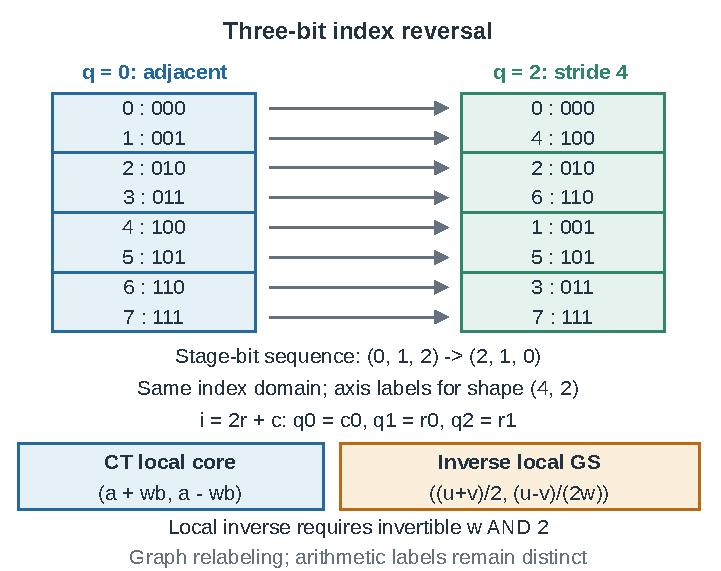
\includegraphics[width=\columnwidth]{figures/drawio/exports/semantic_transport.pdf}
\caption{Reusing the construction through explicit correspondences. Bit
reversal maps the eight-index pairing envelope and its stage-bit sequence.
Axis labels describe the same index domain for a $4\times2$ tensor.
The core inset shows a CT pair and its local inverse GS form, requiring
invertible $w$ and $2$. These are algebraic examples, not claims of identical
floating rounding, arbitrary stage commutation, or equal execution cost.}
\label{fig:semantic-transport}
\end{figure}

Arithmetic labels move separately. A CT pair computes $(a+wb,a-wb)$ and
a GS pair computes $(a+b,w(a-b))$. A GS pair with reciprocal twiddle and
one-half scaling inverts the CT pair where those inverses exist. A full
inverse also reverses stage order and applies the corresponding permutations.
Hadamard changes the local labels to sums and differences, zeta/M\"obius
exchanges one-sided addition and subtraction, and structured stages require
invertible local matrices for inversion. Numerical contracts remain explicit.

For separable power-of-two tensor axes, pairing bits can be labeled by axis
and position. Axis-stage composition then uses the same closure and boundary
rules on the tensor index domain. Axis order and inter-axis layout become
mapping choices subject to the operator's factorization. This describes a
shared construction, not a claim that every multidimensional or arithmetic
variant already has an efficient lowering.

\subsection{Correct composition}
The preceding rules separate the questions of what is computed, where each
value is placed, and when its consumer may run. Their composition must still
implement the requested complete operator.
A composed execution is correct when it covers each required operation once,
each core implements its labels, every handoff preserves value identity, and
every read occurs after production and before storage reuse. A topological
induction suffices. Correct predecessor values reach the next operation through
consistent layouts and valid lifetimes, and its arithmetic produces the
required outputs. Thus local arithmetic, boundary layout, and scheduling
carry distinct correctness obligations. The next section realizes these
obligations with block-level and resident subgraph execution.
